% Provenance (never printed): old seconde/premiere S material on water as a
% resource (stocks and flows of the water cycle, residence times, groundwater,
% overuse as a physical fact); see sources/book2/PROVENANCE.md. Residence
% times are computed in figdata/grade-10/residence_times.py, the Aral Sea
% budget in figdata/grade-10/aral_sea.py.
\chapter{Freshwater Resources}\label{ch:g10:freshwater-resources}

In 1960 the Aral Sea, in the deserts of Central Asia, was the fourth largest
lake in the world. Two great rivers, fed by snow and rain in faraway
mountains, flowed into it; none flowed out. In the 1960s their water was
taken to irrigate the desert. Satellites have watched what followed: the lake
has broken into pieces, and most of its bed is now dry land. The cause,
overwhelmingly, was not a change of climate but the irrigation: the lake
received far less water than evaporation took from it each year. This chapter counts the water of the Earth, where it
is stored and how fast it moves, and shows that a resource of water is above
all a flow: when more is taken from a reservoir than flows into it, the
reservoir empties, at a rate that a simple budget predicts.
% ledger: nasa:aral, gaybullaev:aral-1960, micklin:aral

\begin{omfigure}
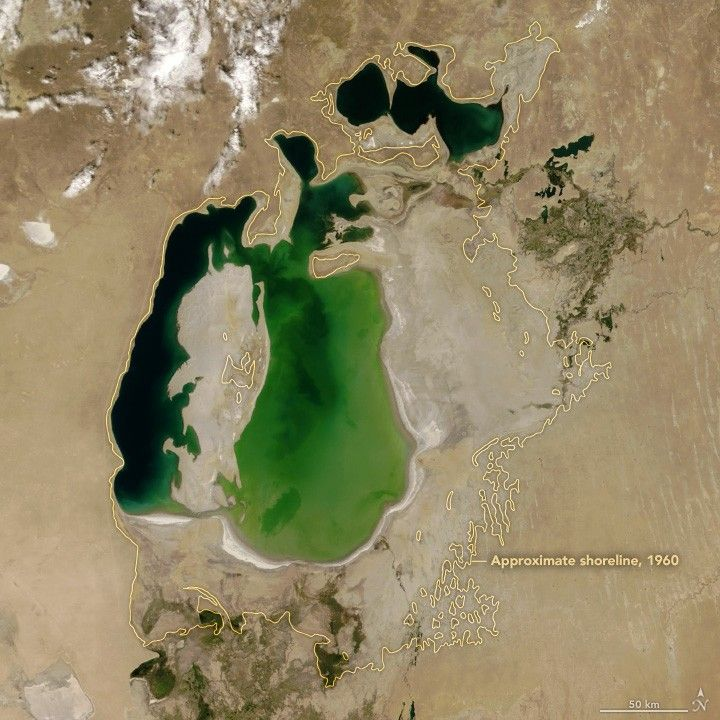
\includegraphics[width=0.47\linewidth]{images/book2/g10-nasa-aral-2000.jpg}\hspace{0.03\linewidth}%
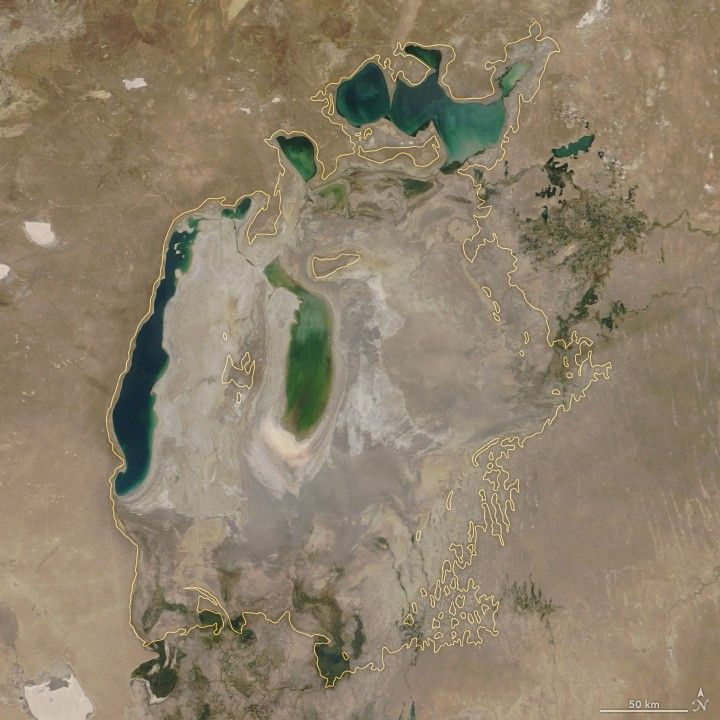
\includegraphics[width=0.47\linewidth]{images/book2/g10-nasa-aral-2018.jpg}

{\small The Aral Sea seen by the MODIS instrument on NASA's Terra satellite in
August 2000 (left) and August 2018 (right); the yellow line is the approximate
shoreline of 1960. The scale bar is \qty{50}{km}. Images: NASA Earth
Observatory.}
\end{omfigure}

\begin{recall}
The water cycle moves water between the ocean, the air and the land:
evaporation, condensation into clouds, precipitation, runoff; the total mass
of water is conserved (the physics books). Rocks with connected pores are
permeable; below the water table their pores are full of water, and a layer
that holds and lets through enough water to feed wells is an aquifer
(Book 1, grade 6). Most of the Earth's water is salt water (Book 1,
grade 2). A river carries away the water of its \omterm{def:g10:drainage-basins:drainage-basin}{drainage basin}; its \omterm{def:g10:drainage-basins:discharge}{discharge}
is a volume per second (\cref{ch:g10:drainage-basins}).
\end{recall}

\section{Where the water is}

The Earth holds about 1.39 billion cubic kilometres of water. Almost all of it
is in the ocean; only \qty{2.5}{\percent} is fresh. And most of that fresh
water is out of reach: more than two-thirds of it is frozen in the ice caps
and glaciers, and almost a third lies underground.
% ledger: usgs:water-stocks

\begin{center}
\small
\begin{tabular}{|l|r|r|}
\hline
\textbf{reservoir} & \textbf{volume (\unit{km^3})} & \textbf{share of fresh water} \\ \hline
oceans, seas and bays & \num{1338000000} & (salt) \\ \hline
ice caps, glaciers and permanent snow & \num{24064000} & \qty{68.7}{\percent} \\ \hline
fresh groundwater & \num{10530000} & \qty{30.1}{\percent} \\ \hline
ground ice and permafrost & \num{300000} & \qty{0.86}{\percent} \\ \hline
fresh lakes & \num{91000} & \qty{0.26}{\percent} \\ \hline
soil moisture & \num{16500} & \qty{0.05}{\percent} \\ \hline
atmosphere & \num{12900} & \qty{0.04}{\percent} \\ \hline
rivers & \num{2120} & \qty{0.006}{\percent} \\ \hline
\end{tabular}

{\small One estimate of the world's water, after Shiklomanov (1993), from the
U.S. Geological Survey. Saline groundwater (\num{12870000}~\unit{km^3}) and
saline lakes are left out.}
\end{center}
% ledger: usgs:water-stocks

Rivers and fresh lakes, from which people draw most of the water they use,
together hold less than one hundredth of one per cent of all the water. Yet
rivers never run dry for long: they are not a store but a flow, refilled by
every rain.

\section{Stocks and fluxes}

\begin{definition}[Stock; flux]\label{def:g10:freshwater-resources:stock}
In a budget of water, a \emph{stock}\index{stock (of water)} is the amount
of water held in a reservoir --- the ocean, the air, the ice, an aquifer, a
lake --- at a given time, as a volume or a mass. A
\emph{flux}\index{flux (of water)} is the amount that passes from one reservoir to another per unit
time, for example in cubic kilometres per year.
\end{definition}

A \omterm{def:g10:freshwater-resources:stock}{stock} changes only through its \omterm{def:g10:freshwater-resources:stock}{fluxes}: what enters minus what leaves. When
the two are equal, the \omterm{def:g10:freshwater-resources:stock}{stock} is in \emph{steady state}: it stays the same
although its water is always being replaced.

\begin{omfigure}
\begin{tikzpicture}[font=\footnotesize, >={Stealth[length=6pt]}]
  % ocean, land, atmosphere
  \fill[omSea] (0,0) rectangle (6.4,1.6);
  \fill[omLithAlluv] (6.4,0) -- (6.4,1.6) -- (8.2,2.1) -- (10.4,2.6) -- (12,2.9) -- (12,0) -- cycle;
  \fill[omLithSand!60] (6.4,0) -- (12,0) -- (12,1.0) -- (6.4,0.7) -- cycle;
  \draw[black!50] (6.4,1.6) -- (8.2,2.1) -- (10.4,2.6) -- (12,2.9);
  \fill[omIce] (10.6,2.65) -- (11.3,3.35) -- (12,2.9) -- cycle;
  \node[align=center] at (3.2,0.75) {\textbf{ocean}\\\num{1335040}};
  \node[align=center] at (9.3,1.35) {soil moisture 122\\lakes and rivers 178};
  \node[align=center] at (9.3,0.35) {groundwater \num{15300}};
  \node[align=center] at (11.2,2.25) {ice\\\num{26350}};
  % atmosphere
  \draw[black!30, rounded corners=8pt, fill=omWxCloud] (1.0,4.6) rectangle (11.0,5.6);
  \node[align=center] at (6.0,5.1) {\textbf{atmosphere} 12.7};
  % fluxes
  \draw[->, omProp, line width=1.4pt] (1.4,1.7) -- node[left, align=right] {evaporation\\413} (1.4,4.5);
  \draw[->, omWxRain, line width=1.4pt] (4.4,4.5) -- node[pos=0.3, right, align=left] {precipitation\\373} (4.4,1.7);
  \draw[->, omWxRain, line width=1.4pt] (7.6,4.5) -- node[pos=0.7, left, align=right] {precipitation\\113} (7.6,2.05);
  \draw[->, omProp, line width=1.4pt] (10.0,2.6) -- node[right, align=left] {evaporation and\\transpiration 73} (10.0,4.5);
  \draw[->, black!60, line width=1.2pt] (4.9,5.85) -- node[above] {water vapour carried over the land: 40} (7.4,5.85);
  \draw[->, omRiver, line width=1.4pt] (7.6,1.2) -- node[above, inner sep=2pt] {runoff 40} (6.0,1.2);
\end{tikzpicture}

{\small The global water cycle of the 1990s (schematic; not to scale). \omterm{def:g10:freshwater-resources:stock}{Stocks}
in thousands of \unit{km^3}, \omterm{def:g10:freshwater-resources:stock}{fluxes} in thousands of \unit{km^3} per year.
After Trenberth and others (2007). Estimates of the \omterm{def:g10:freshwater-resources:stock}{stocks} differ from one
study to another: compare the groundwater and ice here with the table above.}
\end{omfigure}
% ledger: trenberth:water-cycle

The cycle is balanced. Each year the ocean loses \num{413000}~\unit{km^3} by
evaporation and gets back \num{373000} as rain and snow and \num{40000} from
the rivers. The air receives $413\,000 + 73\,000 = \num{486000}$~\unit{km^3}
and gives back $373\,000 + 113\,000$, the same. The land receives
\num{113000}~\unit{km^3} of precipitation; \num{73000} return to the air by
evaporation and through the leaves of plants, and the remaining \num{40000}
run off to the sea, in rivers and underground.
% ledger: trenberth:water-cycle

\begin{definition}[Renewable fresh water]\label{def:g10:freshwater-resources:renewable}
The \emph{renewable fresh water}\index{renewable fresh water} of a region is
the \omterm{def:g10:freshwater-resources:stock}{flux} of fresh water renewed each year by precipitation, which flows
through it as runoff in rivers and as groundwater. It is a \omterm{def:g10:freshwater-resources:stock}{flux}, in cubic
kilometres per year, not a \omterm{def:g10:freshwater-resources:stock}{stock}.
\end{definition}

For all the land of the Earth, it is the \num{40000}~\unit{km^3} that reach
the sea each year. A region can use its renewable water year after year
without running short. What it takes beyond it can only come from a \omterm{def:g10:freshwater-resources:stock}{stock},
which then shrinks.

\section{Residence time}

How long does a molecule of water stay in a reservoir? Some leave at once,
others stay much longer; but on average, the answer follows from the \omterm{def:g10:freshwater-resources:stock}{stock} and
the \omterm{def:g10:freshwater-resources:stock}{flux} alone.

\begin{definition}[Residence time]\label{def:g10:freshwater-resources:residence-time}
The \emph{residence time}\index{residence time} of water in a reservoir is the
average time that water spends in it between entering and leaving.
\end{definition}

\begin{proposition}[Residence time, stock and flux]\label{prop:g10:freshwater-resources:residence}
For a reservoir in steady state, holding a \omterm{def:g10:freshwater-resources:stock}{stock} $S$ crossed by a \omterm{def:g10:freshwater-resources:stock}{flux} $F$
(in and out), the \omterm{def:g10:freshwater-resources:residence-time}{residence time} is
\[
T = \frac{S}{F}.
\]
\end{proposition}

\begin{proof}
In steady state, a volume $F$ enters and a volume $F$ leaves each year, while
the \omterm{def:g10:freshwater-resources:stock}{stock} stays $S$. After a time $S/F$, a volume $F \times S/F = S$ has
entered: as much as the whole reservoir holds. On average, the water present at
the start has then been replaced, so the water stays $S/F$ in the reservoir.
\end{proof}

\begin{example}[Water in the air]\label{ex:g10:freshwater-resources:atmosphere}
The atmosphere holds \num{12700}~\unit{km^3} of water, and
\num{486000}~\unit{km^3} fall out of it each year as rain and snow. Its
\omterm{def:g10:freshwater-resources:residence-time}{residence time} is $12\,700/486\,000 \approx \num{0.026}$ year, about
\num{9.5} days: the water of the air is renewed every week or two. A cloud
that rains today is made of water that left the ocean or the ground a few
days ago.
\end{example}
% ledger: trenberth:water-cycle (t_atmosphere_days 9.5 in figdata/grade-10/residence_times.py)

The same computation gives about \num{19} days for the water in river
channels ($2120$~\unit{km^3} carried by \num{40000}~\unit{km^3} a year), a few
years for lakes and rivers together, and about \num{3200} years for the ocean
($1\,335\,040/413$ thousand~\unit{km^3}). Groundwater can be slower still: the
deepest water of some aquifers is hundreds of thousands of years old.
% ledger: trenberth:water-cycle, usgs:water-stocks, sturchio:nubian-age

\begin{omfigure}
\begin{tikzpicture}
\begin{axis}[omrecord, xbar, xmode=log, log origin=infty, width=0.74\linewidth, height=5.6cm,
  xmin=1, xmax=1e9, ymin=-0.6, ymax=4.6, bar width=11pt,
  ytick={0,1,2,3,4}, yticklabels={atmosphere, rivers, {lakes and rivers}, ocean, {deep groundwater (age)}},
  xtick={1,30.44,365.25,36525,3652500,365250000}, xticklabels={1 day, 1 month, 1 year, 100 years, \num{10000} years, 1 million years},
  xticklabel style={font=\scriptsize, rotate=25, anchor=north east}, yticklabel style={font=\small},
  xlabel={residence time (logarithmic scale)}, label style={font=\small}, xmajorgrids]
\addplot[fill=omDef!45, draw=omDef!80!black] table[x=days, y=idx] {figdata/out/grade-10-residence_times-times.dat};
\draw[fill=omProp!45, draw=omProp!80!black] (axis cs:73050000,3.75) rectangle (axis cs:365250000,4.25);
\node[anchor=west, font=\scriptsize] at (axis cs:9.5,0) {\num{9.5} days};
\node[anchor=west, font=\scriptsize] at (axis cs:19.4,1) {\num{19} days};
\node[anchor=west, font=\scriptsize] at (axis cs:1625,2) {\num{4.5} years};
\node[anchor=west, font=\scriptsize] at (axis cs:1180690,3) {\num{3200} years};
\node[anchor=east, font=\scriptsize] at (axis cs:73050000,4) {\num{200000} to 1 million years};
\end{axis}
\end{tikzpicture}

{\small \omterm{def:g10:freshwater-resources:residence-time}{Residence times} of water, computed as \omterm{def:g10:freshwater-resources:stock}{stock} divided by \omterm{def:g10:freshwater-resources:stock}{flux} from the
global water cycle (blue), and the measured age of deep groundwater under the
eastern Sahara (orange). Logarithmic axis: from one year on, each marked step is a hundredfold. Data:
Trenberth and others (2007); U.S. Geological Survey; Sturchio and others
(2004).}
\end{omfigure}
% values computed in figdata/grade-10/residence_times.py

\omterm{def:g10:freshwater-resources:residence-time}{Residence time} measures how fast a reservoir recovers. Water taken from a
river is replaced in days; a polluted or emptied lake takes years; groundwater
that took thousands of years to gather is, on the scale of a human life, not
renewed at all.

\begin{method}[A water budget]\label{met:g10:freshwater-resources:budget}
\begin{enumerate}
  \item Choose the reservoir: a lake, an aquifer, a basin, the air.
  \item List every \omterm{def:g10:freshwater-resources:stock}{flux} into it (rivers, rain, seepage) and out of it
        (rivers, evaporation, pumping), in the same unit.
  \item The change of the \omterm{def:g10:freshwater-resources:stock}{stock} per year is the sum of the inputs minus the
        sum of the outputs.
  \item If the \omterm{def:g10:freshwater-resources:stock}{stock} does not change, inputs equal outputs, and the \omterm{def:g10:freshwater-resources:residence-time}{residence
        time} is the \omterm{def:g10:freshwater-resources:stock}{stock} divided by either.
\end{enumerate}
\end{method}

\section{Aquifers as reservoirs}

Rain that soaks into the ground and reaches the water table \emph{recharges}
the aquifer below. The water then moves slowly through the pores of the rock,
towards springs, rivers or the sea. Where a
permeable layer dips under an impermeable one, such as clay, its water is
\emph{confined}: it is fed only where the layer reaches the surface, which may
be far away.

\begin{omfigure}
\begin{tikzpicture}[font=\footnotesize, >={Stealth[length=5pt]}]
  % layers dipping to the right
  \fill[lith shale] (0,0) -- (12,0) -- (12,0.8) -- (0,2.4) -- cycle;
  \fill[lith sandstone] (0,2.4) -- (12,0.8) -- (12,2.2) -- (2.2,3.5) -- (0,3.8) -- cycle;
  \fill[lith shale] (2.2,3.5) -- (12,2.2) -- (12,3.4) -- (3.6,3.9) -- cycle;
  % ground surface
  \draw[line width=0.8pt, brown!60!black] (0,3.8) -- (1.2,4.0) -- (2.2,3.9) -- (3.6,3.9) -- (6,3.6) -- (9,3.5) -- (12,3.4);
  \fill[omLithAlluv] (0,3.8) -- (1.2,4.0) -- (2.2,3.9) -- (2.2,3.5) -- (0,3.8) -- cycle;
  \fill[omLithAlluv] (2.2,3.9) -- (3.6,3.9) -- (2.2,3.5) -- cycle;
  \fill[omLithAlluv] (3.6,3.9) -- (6,3.6) -- (9,3.5) -- (12,3.4) -- (3.6,3.9) -- cycle;
  % water table in the unconfined part
  \draw[omDef, line width=1pt, dashed] (0,3.3) .. controls (1.0,3.35) and (1.8,3.2) .. (2.6,3.45);
  \node[anchor=south west, text=omDef, fill=white, fill opacity=0.8, text opacity=1, inner sep=1pt] at (0.05,2.75) {water table};
  % rain and recharge
  \foreach \x in {0.35,0.65,0.95,1.25} \draw[omWxRain, thick] (\x,4.9) -- (\x-0.15,4.4);
  \node[anchor=south, text=omWxRain] at (0.7,4.95) {rain: recharge};
  % flow arrows in the aquifer
  \draw[->, omDef, line width=1.1pt] (2.0,2.85) -- (4.4,2.55);
  \draw[->, omDef, line width=1.1pt] (5.4,2.4) -- (7.8,2.1);
  \draw[->, omDef, line width=1.1pt] (8.8,1.95) -- (11.2,1.65);
  % wells
  \draw[black!70, line width=1.6pt] (1.95,3.95) -- (1.95,2.9);
  \node[anchor=south] at (1.95,4.0) {well};
  \draw[black!70, line width=1.6pt] (7.0,3.55) -- (7.0,1.9);
  \node[anchor=south] at (7.0,3.6) {well};
  % labels
  \node[align=center, fill=white, fill opacity=0.85, text opacity=1, inner sep=1.5pt] at (1.5,0.8) {impermeable clay};
  \node[align=center, fill=white, fill opacity=0.85, text opacity=1, inner sep=1.5pt] at (8.6,2.95) {impermeable clay};
  \node[anchor=north, align=center] at (1.6,-0.1) {unconfined aquifer:\\recharge area};
  \node[anchor=north, align=center] at (6.4,-0.1) {confined aquifer};
  \node[anchor=north, align=center] at (10.6,-0.1) {old water, far from\\the recharge area};
\end{tikzpicture}

{\small An aquifer in a permeable sandstone (schematic). Rain recharges it
where it reaches the surface; there the water table is free to rise and fall.
Farther on, under the clay, the aquifer is confined, and its water moves
slowly down the layer: the farther from the recharge area, the older the
water.}
\end{omfigure}

\begin{definition}[Fossil groundwater]\label{def:g10:freshwater-resources:fossil-groundwater}
\emph{Fossil groundwater}\index{fossil groundwater} is groundwater that
entered its aquifer long ago, often under a wetter climate, and that today's
recharge does not renew on the scale of human lifetimes.
\end{definition}

Under the eastern Sahara lies a vast sandstone aquifer. Its deepest water,
dated by the decay of a rare radioactive form of krypton, is
\num{200000} to a million years old. It flowed in slowly from a recharge area
in south-western Egypt, and its chemistry shows that it fell as rain during
past wet periods of the ice ages, when moist air from the Atlantic reached
the region. Pumped today, such water is a \omterm{def:g10:freshwater-resources:stock}{stock} being mined, not a flow.
% ledger: sturchio:nubian-age

When pumping exceeds recharge, the water table falls. In the High Plains of
the central United States, the aquifer under some \num{175000} square miles
(\qty{453000}{km^2}) has been pumped for irrigation since about 1950. By 2015
its water level had fallen by \qty{4.8}{m} on average, and by up to
\qty{71}{m} (234 feet) in some wells; the aquifer had lost about
\num{273} million acre-feet of water, some \qty{340}{km^3}.
% ledger: mcguire:high-plains (1 acre-foot = 1233.5 m3)

\begin{omfigure}
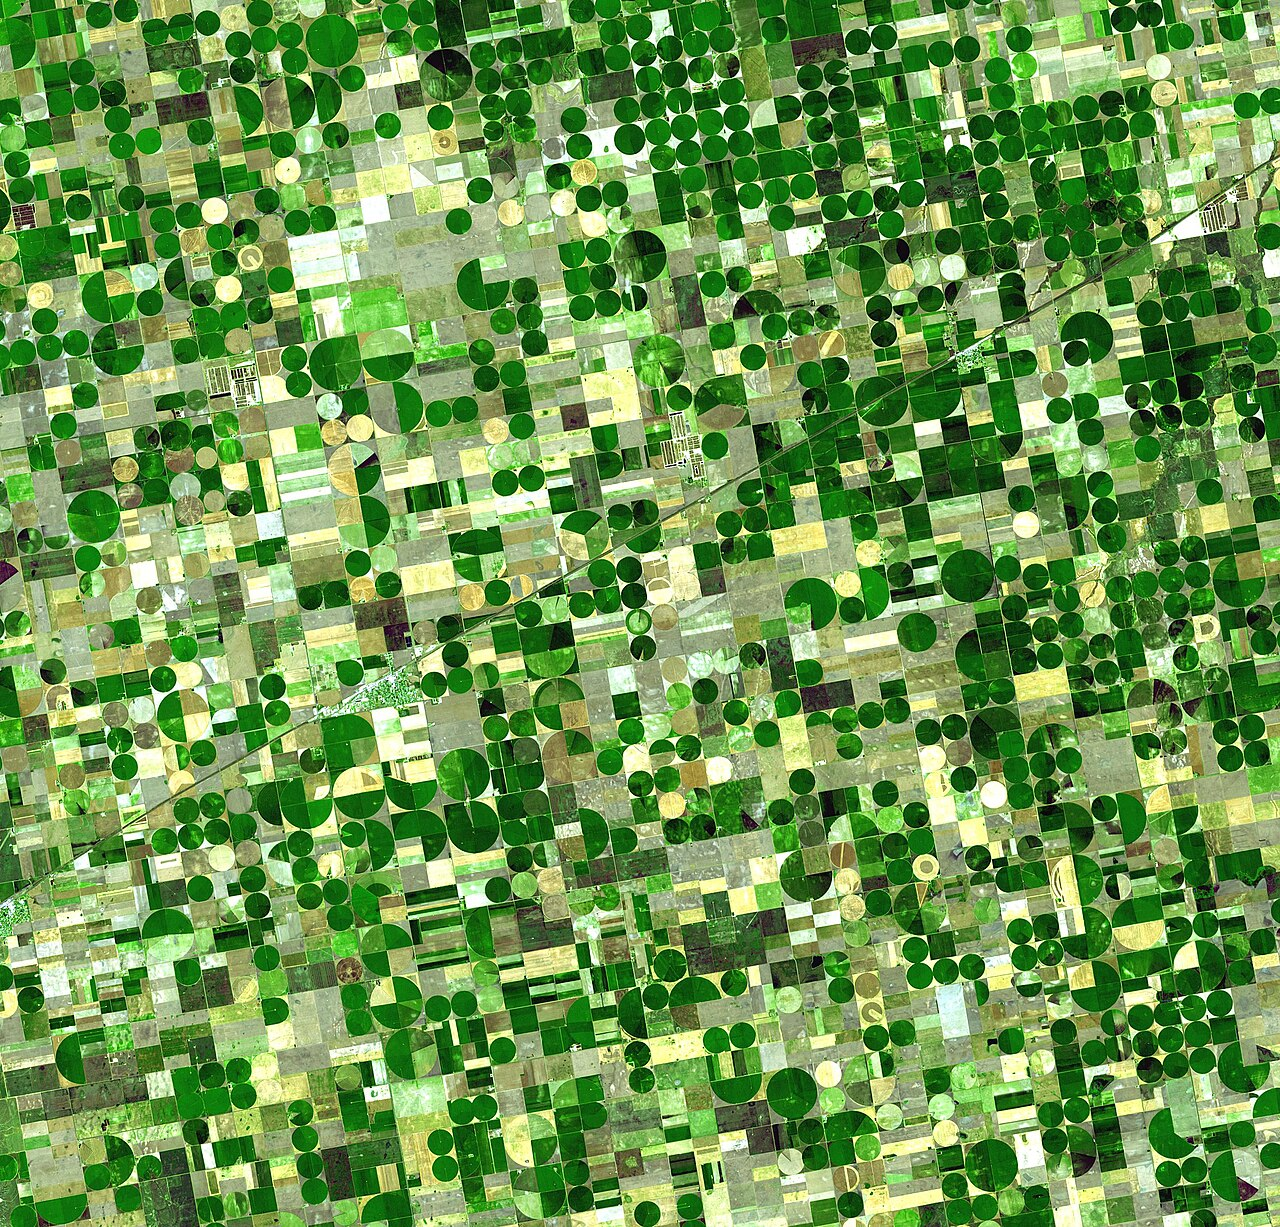
\includegraphics[width=0.5\linewidth]{images/book2/g10-nasa-kansas-center-pivot.jpg}

{\small Irrigated fields near Sublette, Kansas, seen by the ASTER instrument on
NASA's Terra satellite in June 2001 (about \qty{37}{km} across). Each circle
is a field watered by a long sprinkler arm turning about its centre; the
circles are \num{800} and \qty{1600}{m} across. Image: NASA (public domain).}
\end{omfigure}

Groundwater cannot be seen from space, but it can be weighed: two satellites
flying one behind the other feel the slight changes in the Earth's pull caused
by the mass of water that comes and goes below them, and map where the \omterm{def:g10:freshwater-resources:stock}{stock}
of water on land rises and falls from month to month.

\begin{omfigure}
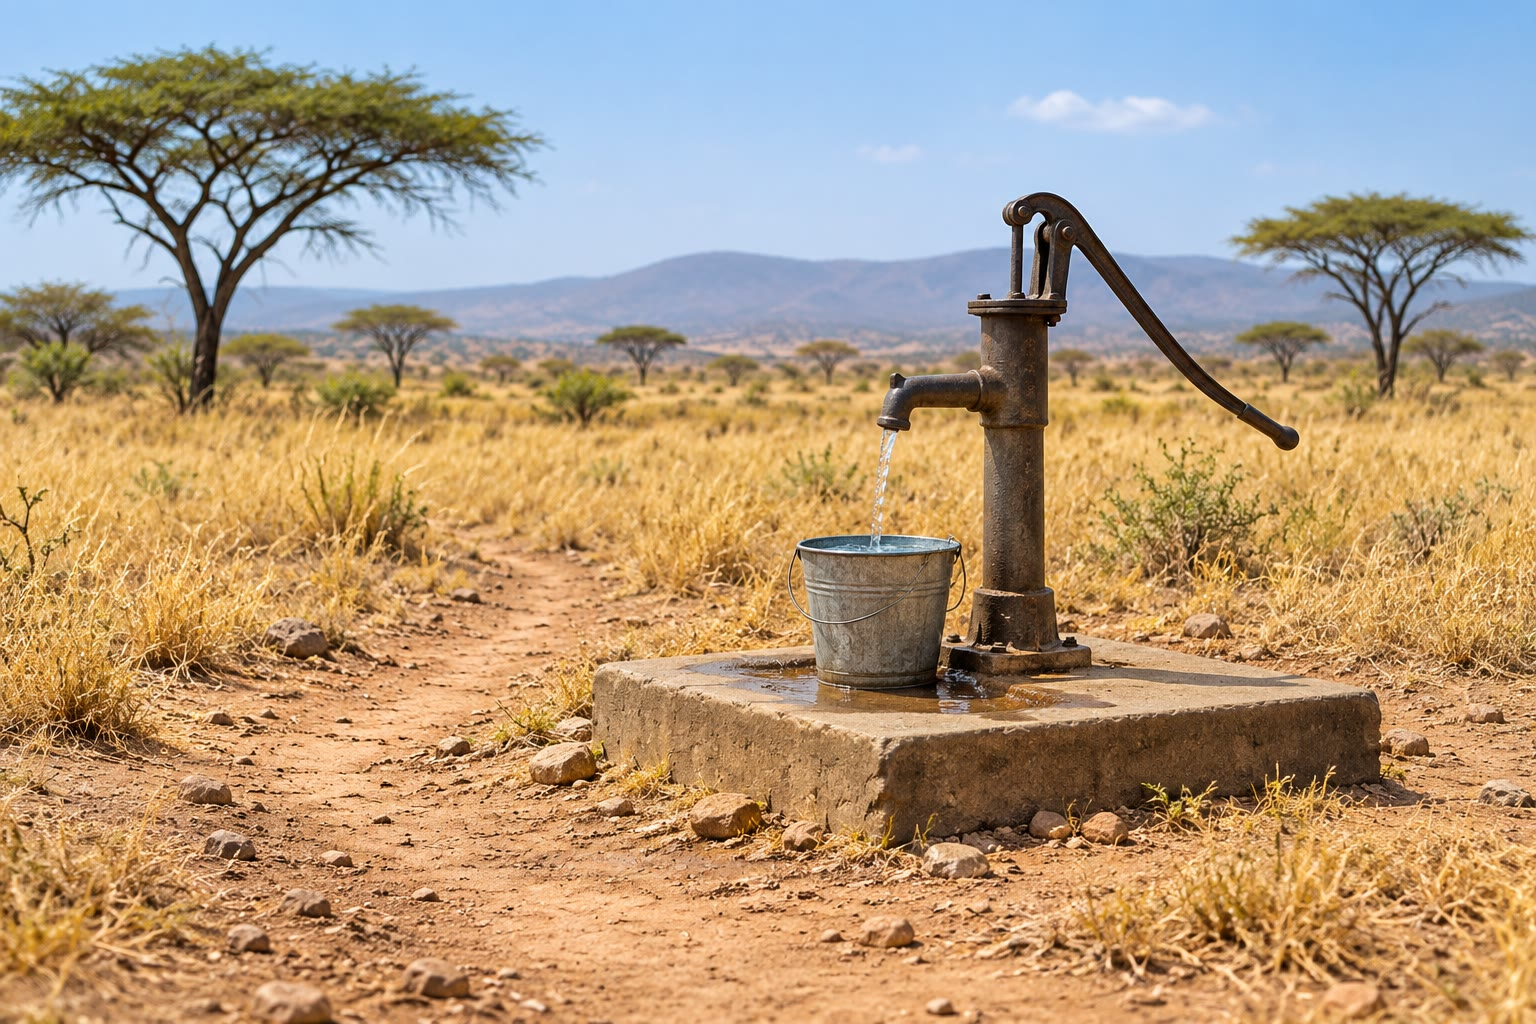
\includegraphics[width=0.55\linewidth]{images/book2/ai/g10-hand-pump-well.jpg}

{\small A hand pump on a well in a dry landscape: the water drawn here comes
from the ground below, out of reach of the dry season.}
\end{omfigure}

\section{Overuse as a physical fact}

The Aral Sea has no outlet: the water of its two rivers, the Amu Darya and
the Syr Darya, leaves only by evaporation. In 1960 it covered
\qty{68000}{km^2}, held \qty{1093}{km^3} and its water contained \qty{10}{g}
of salt per litre. That year evaporation removed \qty{71.1}{km^3}, and rain
on the lake brought \qty{9.4}{km^3}: to keep its level, the lake needed
$71.1 - 9.4 = \qty{61.7}{km^3}$ a year from its rivers.
% ledger: gaybullaev:aral-1960, gaybullaev:aral-table

From the 1960s the rivers were diverted to irrigate the desert, and almost
none of their water reached the lake: in the 1970s and 1980s, often less
than \qty{2}{km^3} a year. Evaporation went on, and the lake
began to shrink. Its budget sets how fast. Evaporation takes a layer of water
whose thickness depends on the climate, here about a metre a year
($71.1/68\,000 \approx \qty{0.00105}{km}$). If the inflow stops, the level
falls by about that much each year, less the rain. As the lake shrinks, its
area and so its evaporation shrink too, and the fall slows down; but it does
not stop until the inflow and the evaporation balance again.
% ledger: gaybullaev:aral-table (values computed in figdata/grade-10/aral_sea.py)

\begin{omfigure}
\begin{tikzpicture}
\begin{axis}[omrecord, name=vol, width=0.46\linewidth, height=5.4cm, xmin=1955, xmax=2012, ymin=0, ymax=1200,
  xtick={1960,1980,2000}, xticklabel style={/pgf/number format/1000 sep={}}, scaled y ticks=false,
  ylabel={volume (\unit{km^3})}, xlabel={year}, tick label style={font=\small}, label style={font=\small},
  title={\small water volume}]
\addplot[omDef, line width=1pt, mark=*, mark size=1.3pt] table[x=year, y=volume] {figdata/out/grade-10-aral_sea-record.dat};
\end{axis}
\begin{axis}[omrecord, at={(vol.east)}, anchor=west, xshift=1.4cm, width=0.46\linewidth, height=5.4cm,
  xmin=1955, xmax=2012, ymin=0, ymax=140, xtick={1960,1980,2000},
  xticklabel style={/pgf/number format/1000 sep={}},
  ylabel={salinity (\unit{g/L})}, xlabel={year}, tick label style={font=\small}, label style={font=\small},
  title={\small salinity}]
\addplot[omProp, line width=1pt, mark=*, mark size=1.3pt] table[x=year, y=salinity] {figdata/out/grade-10-aral_sea-record.dat};
\end{axis}
\end{tikzpicture}

{\small The Aral Sea from 1960 to 2010: the volume of its water fell to a
tenth, while the salt left behind by evaporation grew thirteen times more
concentrated. Data: Gaybullaev and others (2012).}
\end{omfigure}
% ledger: gaybullaev:aral-table

By 2010 the lake held \qty{98}{km^3}, a tenth of its 1960 volume, over
\qty{14280}{km^2}; its salinity had reached \qty{130}{g/L}, far saltier than
the ocean. Its level had fallen by more than \qty{20}{m}. Salty dust blows
from the dry bed. The cause is not hidden: the inflow of the lake was cut
while its evaporation was not.
% ledger: gaybullaev:aral-table, gaybullaev:aral-1960, micklin:aral, nasa:aral

\section{Exercises}

\begin{exercise}[$\star$]\label{exo:g10:freshwater-resources:1}
Define a \omterm{def:g10:freshwater-resources:stock}{stock}, a \omterm{def:g10:freshwater-resources:stock}{flux} and a \omterm{def:g10:freshwater-resources:residence-time}{residence time}, and give the units of each.
\end{exercise}

\begin{exercise}[$\star$]\label{exo:g10:freshwater-resources:2}
From the table of the world's water: what share of all water is fresh? Of the
fresh water, what shares are frozen and underground? Which reservoir holds
the least?
\end{exercise}

\begin{exercise}[$\star$]\label{exo:g10:freshwater-resources:3}
Define \omterm{def:g10:freshwater-resources:renewable}{renewable fresh water} and \omterm{def:g10:freshwater-resources:fossil-groundwater}{fossil groundwater}. Why is the first a \omterm{def:g10:freshwater-resources:stock}{flux}
and the second a \omterm{def:g10:freshwater-resources:stock}{stock}?
\end{exercise}

\begin{exercise}[$\star$]\label{exo:g10:freshwater-resources:4}
How many times more water do the world's fresh lakes (\num{91000}~\unit{km^3})
hold than its rivers (\num{2120}~\unit{km^3})?
\end{exercise}

\begin{exercise}[$\star$]\label{exo:g10:freshwater-resources:5}
On the chart of \omterm{def:g10:freshwater-resources:residence-time}{residence times}, which reservoir renews its water fastest,
and which slowest? How many times longer does water stay in the ocean than in
the air?
\end{exercise}

\begin{exercise}[$\star\star$]\label{exo:g10:freshwater-resources:6}
The atmosphere holds \num{12700}~\unit{km^3} of water. Compute its \omterm{def:g10:freshwater-resources:residence-time}{residence
time} from the evaporation that enters it (\num{413000} from the ocean and
\num{73000}~\unit{km^3} from the land each year), and check that it matches
the \omterm{def:g10:freshwater-resources:residence-time}{residence time} computed from the precipitation that leaves it.
\end{exercise}

\begin{exercise}[$\star\star$]\label{exo:g10:freshwater-resources:7}
The ocean holds \num{1335040} thousand~\unit{km^3} and loses
\num{413} thousand~\unit{km^3} a year by evaporation. Compute its \omterm{def:g10:freshwater-resources:residence-time}{residence
time}. Why is it the same if computed with what enters it?
\end{exercise}

\begin{exercise}[$\star\star$]\label{exo:g10:freshwater-resources:8}
Using the \omterm{def:g10:freshwater-resources:stock}{fluxes} of the global water cycle, write the budget of the land: what
falls on it, what returns to the air, what runs off. What share of the rain
falling on land returns to the air?
\end{exercise}

\begin{exercise}[$\star\star$]\label{exo:g10:freshwater-resources:9}
The High Plains aquifer lost about \num{273.2} million acre-feet of water from
about 1950 to 2015 (\num{1}~acre-foot = \qty{1233.5}{m^3}). Convert
this volume to \unit{km^3} and compare it with the volume of the Aral Sea in
1987 (\qty{345.6}{km^3}).
\end{exercise}

\begin{exercise}[$\star\star$]\label{exo:g10:freshwater-resources:10}
The average water level of the High Plains aquifer fell by \num{15.8} feet
from about 1950 to 2015 (\num{1}~foot = \qty{0.3048}{m}). What is that in
metres, and in centimetres per year?
\end{exercise}

\begin{exercise}[$\star\star$]\label{exo:g10:freshwater-resources:11}
An aquifer holds \qty{2}{km^3} of water and is recharged with
\qty{0.01}{km^3} a year. What is the \omterm{def:g10:freshwater-resources:residence-time}{residence time} of its water? Wells now
pump \qty{0.05}{km^3} a year from it. Suppose that the recharge goes on and
that the wells are now the only way out for the water: how long will it
last?
\end{exercise}

\begin{exercise}[$\star\star\star$]\label{exo:g10:freshwater-resources:12}
Compute the \omterm{def:g10:freshwater-resources:residence-time}{residence time} of the water of the Aral Sea in 1960
(\qty{1093}{km^3}, evaporation \qty{71.1}{km^3} a year) and in 2010
(\qty{98.1}{km^3}, evaporation \qty{11.4}{km^3} a year). Why did its
evaporation fall?
\end{exercise}

\begin{exercise}[$\star\star\star$]\label{exo:g10:freshwater-resources:13}
A lake with no outlet covers \qty{100}{km^2}. Evaporation removes
\qty{1.2}{m} of water a year from its surface, and rain adds \qty{0.2}{m}.
\begin{enumerate}
  \item What inflow, in \unit{km^3} a year, keeps its level steady?
  \item The inflow is halved. By how much does the level fall in the first
        year?
  \item Why does the fall slow down in the following years?
\end{enumerate}
\end{exercise}

\begin{exercise}[$\star\star\star$]\label{exo:g10:freshwater-resources:14}
In a desert, rain recharges an aquifer with \qty{1}{mm} of water a year.
The aquifer is \qty{100}{m} thick and water fills \qty{20}{\percent} of its
volume. How long would it take the recharge to fill it? Compare with the
age of the deep water of the Sahara aquifer.
\end{exercise}

\begin{exercise}[$\star\star\star$]\label{exo:g10:freshwater-resources:15}
The High Plains aquifer covers about \qty{453000}{km^2} and lost about
\qty{337}{km^3} of water by 2015. What thickness of water, spread over the
whole aquifer, is that? Its water level fell by \qty{4.8}{m} on average.
Why is the fall of the water level larger than the thickness of water lost?
\end{exercise}

\section{Problem: The Aral Sea's Budget}

\begin{problem}[{Weekend problem --- how fast does a lake disappear?}]
\label{pb:g10:freshwater-resources:1}
% ledger: gaybullaev:aral-table, gaybullaev:aral-1960, micklin:aral (values computed in figdata/grade-10/aral_sea.py)
The table gives the budget of the Aral Sea for four years (volumes in
\unit{km^3}, salinity in grams of salt per litre). In 1960 the lake covered
\qty{68000}{km^2}.
\begin{center}
\small
\begin{tabular}{|c|c|c|c|c|c|}
\hline
year & river inflow & rain on the lake & evaporation & volume & salinity \\ \hline
1960 & 42.0 & 9.4 & 71.1 & 1093.0 & 10.0 \\ \hline
1984 & 0.3 & 3.5 & 47.9 & 502.7 & 21.9 \\ \hline
1987 & 1.0 & 6.2 & 36.8 & 345.6 & 25.0 \\ \hline
1989 & 3.1 & 5.3 & 35.3 & 327.2 & 30.0 \\ \hline
\end{tabular}

{\small Data: Gaybullaev and others (2012).}
\end{center}

\medskip
\noindent\textbf{Part I --- The lake in 1960.}
\begin{enumerate}
  \item What was the mean depth of the lake in 1960?
  \item Express its volume in cubic metres.
  \item What mass of salt did it hold, in tonnes?
  \item What was the \omterm{def:g10:freshwater-resources:residence-time}{residence time} of its water, counted with evaporation?
  \item Why can a lake with no outlet only lose water by evaporation (and
        seepage)?
\end{enumerate}

\medskip
\noindent\textbf{Part II --- What the lake needs.}
\begin{enumerate}[resume]
  \item What thickness of water did evaporation remove from the lake in
        1960, in metres?
  \item What thickness did the rain add?
  \item What river inflow would have balanced evaporation and rain exactly?
  \item The two rivers carry on average about \qty{79}{km^3} and
        \qty{37}{km^3} a year out of the mountains. What share of this would
        the lake need?
\end{enumerate}

\medskip
\noindent\textbf{Part III --- The lake in the late 1980s.}
\begin{enumerate}[resume]
  \item Write the budget of 1987: inputs, outputs, net change.
  \item Between 1984 and 1989 the volume fell from \qty{502.7}{km^3} to
        \qty{327.2}{km^3}. What was the average fall per year? Compare with
        the budget of 1987.
  \item Assume that a square kilometre of lake loses as much water by
        evaporation as in 1960. What was the area of the lake in 1987?
  \item What share of its 1960 area is that?
  \item Why had evaporation fallen from \qty{71.1}{km^3} to
        \qty{36.8}{km^3}?
  \item What share of its 1960 volume did the lake still hold in 1987?
\end{enumerate}

\medskip
\noindent\textbf{Part IV --- The salt and the level.}
\begin{enumerate}[resume]
  \item If all the salt of 1960 had stayed in the water, what would the
        salinity have been in 1987?
  \item The table gives \qty{25.0}{g/L}. What does the difference suggest?
  \item With no inflow and no rain at all, by how much would the level fall
        each year?
  \item In 1987, how much did the rivers and the rain add, as a thickness
        over the area of question 12?
  \item By how much did the level of the Aral Sea fall in 1987?
\end{enumerate}
\end{problem}
